\part{Processus de Markov \` a temps discret}
\section{Définitions}
\Def{Processus}{Un processus est un phénomène aléatoire qui se déroule au cours du temps.

\bigskip
Si on a un processus, son état à la date $t$ est donné par une variable aléatoire notée par exemple $X_t$\\
$X_t(\omega)=$ l'état du processus à la date $t$ si le hasard est $\omega\in\Omega$.}

L'ensemble des temps peut être :
\begin{itemize}
	\item discret : $\{0,...,n\}$ ou $\mathbb{N}$\\
		Ce ne sont  pas forcément des dates, mais par exemple des numéros d'épreuves.
	\item continu : $[0,T]$ ou $\mathbb{R}^+$
\end{itemize}

\bigskip
Dans ce cours, les processus auront leurs états dans un ensemble fini ou parfois dénombrable $E$, appelé l'espace d'états. Ainsi, on note :
\[X=(X_t)_{t\in T}\]

\Def{Propriété de Markov}{On dit qu'un processus décrit par $X=(X_t)_{t\in T}$ a la propriété de Markov si :
	\[\forall 0\leq t_0<...<t_n<t,\ \mathcal{L}(X_t|X_{t_n},...,X_{t_0})=\mathcal{L}(X_t|X_{t_n})\]
}

\Def{Homogène}{On dit que le processus a la propriété de Markov homogène s'il a la propriété de Markov et, $\forall s<t$ : 
	\[\mathcal{L}(X_t|X_s=x)=\mathcal{L}(X_{t-s}|X_0=x)\]
}

\subsection{Formalisme matriciel}
$E$ est ici considéré comme fini (ou dénombrable), $E=\{i,j,...,k,...\}$
\Def{Différents vecteurs}{\begin{itemize}
	\item Une mesure de probabilité $\mu$ sur $E$ va être représenté par un vecteur ligne, et qu'on notera $\mu$ :
		\[\mu=(\mu_j)_{j\in E} \text{ où } \mu_j=\mu(\{j\})\]
	\item Une fonction $f:E\to\mathbb{R}$ (ou $\mathbb{C}$) sera représenté par un vecteur colonne qui sera noté f :
		\[f=(f^i)_{i\in E} \text{ où } f^i=f(i)\]
\end{itemize}}

\Def{Matrices stochastiques}{L'ensemble des lois $\mathcal{L}(X_t|X_0=i),\ i\in E$ qu'on note $\mathcal{L}(X_t|X_0)$ sera une matrice carrée, notée $\Pi_t$, appelée matrice stochastique.
\begin{itemize}
	\item la ligne $i$ correspondant à la mesure de probabilité \[\mathcal{L}(X_t,X_0=i)=(P_j^i(t))_{j\in E} = (\mathbb{P}(X_t=j|X_0=i))_{j\in E}\]
	\item la colonne $j$ représente la fonction :
		\[i\in E \mapsto P_j^i(t)=\mathbb{P}(X_t=j|X_0=i)\]
\end{itemize}
$\Pi_t$ est une matrice à termes positifs dont la somme de chaque ligne vaut 1.}

\Exemp{}{\begin{eqnarray*}
	\mathbb{E}(f(X_t)|X_0=i)&=&\sum_j f(j)\mathbb{P}(X_t=j|X_0=i)\\
		&=& \sum_j P_j^i(t)f^j\\
		&=& (\Pi_t f)^i
\end{eqnarray*}
Si $\mu_0=\mathcal{L}(X_0)$, $\mu_{0j}=\mathbb{P}(X_0=j)$ 
\begin{eqnarray*}
	\mathbb{E}_{\mu_0}[f(X_t)]&=&\sum_i \mathbb{E}(f(X_t)|X_0=i]\mathbb{P}(X_0=i)\\
				&=&\sum_i \mu_{0i} (\Pi_t f)^i\\
				&=&\mu_0 \Pi_t f
\end{eqnarray*}
et alors si $\mu_t=\mathcal{L}(X_t)$, on a $\mu_t=\mu_0\Pi_t$ (formule de probabilité totale, $\mu_0$ représentant la loi de $X_0$)
\begin{eqnarray*}
	\mathbb{P}(X_t=j)&=&\sum_i \mathbb{P}(X_t=j|X_0=i)\mathbb{P}(X_0=i) \\
			&=& \sum_i \mu_{0,i} P_j^i(t) \\
			&=&(\mu_0\Pi_t)_j
\end{eqnarray*}}

Dans la suite du cours, nous considérerons que nos processus ont toujours la propriété de Markov homogène.
\Theo{Relations de Kolmogorov}{\[\forall s,t\geq 0, \Pi_t\Pi_s=\Pi_s\Pi_t=\Pi_{s+t}\]
\[\Pi_0=I\]}

\begin{dem}
\begin{eqnarray*}
	\forall i,j,\ \mathbb{P}[X_{t+S}=j|X_0=i]&=&\sum_{k\in E} \mathbb{P}(X_{t+s}=j|X_s=k,X_0=i)\mathbb{P}(X_s=k|X_0=i) \\
						&=& \sum_{k\in E} \mathbb{P}(X_{t+s}=j|X_s=k)\mathbb{P}(X_s=k|X_0=i) \text{ Par la propriété de Markov}\\
						&=& \sum_{k\in E} \mathbb{P}(X_t=j|X_0=k) \mathbb{P}(X_j=k|X_0=i) \text{ propriété homogène} \\
				P_j^i(t+s) &=& \sum_{k\in E} P_k^i (s) P_j^k(t) \\
				(\Pi_{t+s})_j^i &=& (\Pi_s\Pi_t)_j^i
\end{eqnarray*}

Donc $\Pi_{t+s}=\Pi_s\Pi_t=\Pi_{s+t}=\Pi_t\Pi_s$.

\[(\Pi_0)_j^i = \mathbb{P}(X_0=i|X_0=j)=\delta_{ij} \Rightarrow \Pi_0=I\]
\end{dem}

\section{Processus de Markov (sous entendu homogène) en temps discret (T=$\mathbb{N}$)}
D'après la relation de Kolmogorov :
\[\Pi_n=(\Pi_1)^n = \Pi^n\]
On note $\Pi_1$ par $\Pi$ la matrice de transition de la chaîne de Markov.\\
On note $P_j^i=\mathbb{P}(X_1=j|X_0=i)$ Ainsi : \[\Pi=[P_j^i]_{i,j\in E}\]

\bigskip
La ligne $i$ de $\Pi_n=\Pi^n=\mathcal{L}(X_n|X_0=i)$\\
Si $\mu_0=\mathcal{L}(X_0)$, alors $\mathcal{L}(X_n)=\mu_0\Pi^n$\\
\[\mathcal{L}(X_0)=(\mathbb{P}(X_0=j))_{j\in E}\]
\[\mathcal{L}(X_n)=\left(\mathbb{P}(X_n=j)\right)_{j\in E}=\left(\sum_{i=1}^n \mathbb{P}(X_n=j|X_0=i)\mathbb{P}(X_0=i)\right)_{j\in E}=\mu_0\Pi^n\]

\subsection{Diagramme de la chaîne de Markov}
C'est un graph orienté dont tous les sommets sont les éléments $i$ de $E$, et les arêtes (orientées) sont définies ainsi : \\
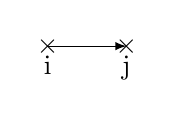
\begin{tikzpicture}
\draw (0,0) node{$\times$} ;
\draw (0,0) node[below]{i} ;
\draw [>=latex,->] (0,0) -- (1,0) ;
\draw (1,0) node{$\times$} ;
\draw (1,0) node[below]{j} ;
\end{tikzpicture}
si et seulement si $p_j^i>0$ ($\mathbb{P}(X_1=j|X_0=i)>0$), ie si et seulement si on peut passer de i à j en une étape.

\subsection{Classification des états}
\Def{Conduire, communiquer et classe d'équivalence}{$i$ peut conduire à $j$ si et seulement si $i=j$ ou s'il existe un chemin allant de $i$ à $j$ (qu'on note $i\rightsquigarrow j$), ie :
\[\exists n\geq 0;\ p_j^i(n)>0\ (\mathbb{P}[X_n=j | X_0=i]>0)\]

Cette relation est un préordre.
\begin{itemize}
	\item réflexive
	\item transitive
\end{itemize}

\bigskip
A l'aide de ce préordre, on construit une relation d'équivalence.\\
"$i$ et $j$ communiquent" (noté $i\leftrightarrow j$) si et seulement si $i\rightsquigarrow j$ et $j\rightsquigarrow i$.
\begin{itemize}
	\item Réflexive
	\item Symétrique
	\item Transitive
\end{itemize}

L'espace d'état est alors partitionné en classes d'équivalence.}

\Exemp{}{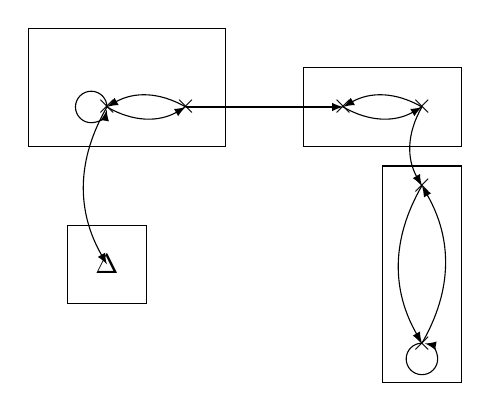
\begin{tikzpicture}
\draw (0,4) node{$\times$} ;
\draw [>=latex,->] (0,4) arc(0:350:0.2) ;
\draw [>=latex,->] (0,4) to[bend right] (1,4) ;
\draw [>=latex,->] (1,4) to[bend right] (0,4) ;
\draw (1,4) node{$\times$} ;
\draw [>=latex,->] (0,4) to[bend right] (0,2) ;
\draw (0,2) node{$\Delta$} ;
\draw [>=latex,->](1,4) to (3,4) ;
\draw (3,4) node{$\times$} ;
\draw [>=latex,->](3,4) to[bend right] (4,4) ;
\draw [>=latex,->](4,4) to[bend right] (3,4) ;
\draw (4,4) node{$\times$} ;
\draw [>=latex,->](4,4) to[bend right] (4,3) ;
\draw [>=latex,->](4,3) to[bend right] (4,1) ;
\draw [>=latex,->](4,1) to[bend right] (4,3) ;
\draw (4,3) node{$\times$} ;
\draw (4,1) node{$\times$} ;
\draw [>=latex,->] (4,1) arc(90:439:0.2) ;
\draw (-1,5) rectangle (1.5,3.5) ;
\draw (-0.5,1.5) rectangle (0.5,2.5) ;
\draw (2.5,4.5) rectangle (4.5,3.5) ;
\draw (4.5,3.25) rectangle (3.5,0.5) ;
\end{tikzpicture}}

Le préordre induit une relation d'ordre sur les classes : $C\rightsquigarrow D \Leftrightarrow \exists i\in C;\ \exists j\in D;\ i\rightsquigarrow j$.\\
Ceci ne dépend pas des $i$ et $j$ choisis.

\bigskip
Si $C\rightsquigarrow D$ et $D\rightsquigarrow C$ alors $C=D$

\Def{Transitoire, finale, ergodique}{\begin{itemize}
\item Une classe est dite transitive si et seulement si elle peut conduire à une autre classe. Ses éléments sont dits transitoires. \\
Tr = Ensemble des états transitoires.
\item Si une classe n'est pas transitoire, on dit qu'elle est finale (elle ne peut conduire qu'à elle-même). Ses éléments sont dits ergodiques.\\
Erg=ensemble des états ergodiques.
\item Si la classe finale n'est composée que d'un élément, on dit qu'il est absorbant ($\Leftrightarrow p_i^i=1$)\\
On le note $\Delta$
\end{itemize}}

\Exemp{}{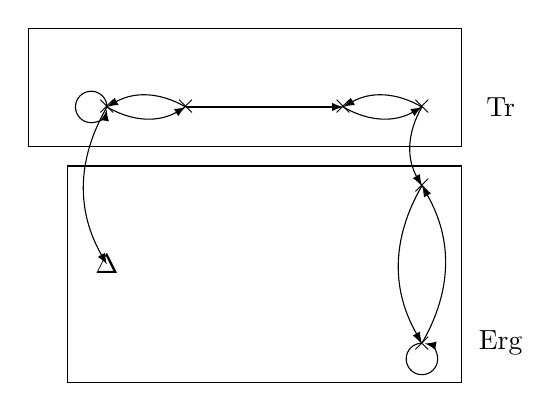
\begin{tikzpicture}
\draw (0,4) node{$\times$} ;
\draw [>=latex,->] (0,4) arc(0:350:0.2) ;
\draw [>=latex,->] (0,4) to[bend right] (1,4) ;
\draw [>=latex,->] (1,4) to[bend right] (0,4) ;
\draw (1,4) node{$\times$} ;
\draw [>=latex,->] (0,4) to[bend right] (0,2) ;
\draw (0,2) node{$\Delta$} ;
\draw [>=latex,->](1,4) to (3,4) ;
\draw (3,4) node{$\times$} ;
\draw [>=latex,->](3,4) to[bend right] (4,4) ;
\draw [>=latex,->](4,4) to[bend right] (3,4) ;
\draw (4,4) node{$\times$} ;
\draw [>=latex,->](4,4) to[bend right] (4,3) ;
\draw [>=latex,->](4,3) to[bend right] (4,1) ;
\draw [>=latex,->](4,1) to[bend right] (4,3) ;
\draw (4,3) node{$\times$} ;
\draw (4,1) node{$\times$} ;
\draw [>=latex,->] (4,1) arc(90:439:0.2) ;
\draw (-1,5) rectangle (4.5,3.5) ;
\draw (-0.5,3.25) rectangle (4.5,0.5) ;
\draw (5,4) node{Tr} ;
\draw (5,1) node{Erg} ;
\end{tikzpicture}}

\Theo{}{Si E est fini, il existe toujours des classes finales, et toute classe transitoire peut conduire à au moins une classe finale (évident)}

\underline{Remarque :} Si E est infini, c'est faux. Prendre par exemple $E=\mathbb{N}$, où chaque $n\in\mathbb{N}$ forme une classe $\{n\}$, elles sont toutes transitoires.

\Def{Forme canonique de la matrice de transition}{On regroupe les états par classe, en mettant d'abord les classes finales. Par exemple, si on considère $C_1$ et $C_2\in$Erg et $C_3$, $C_4$ et $C_5\in$Tr : 
\[\bordermatrix{&C_1 & C_2 & C_3 & C_4 & C_5\cr
C_1 & A_1 &  0  & |0 & 0 & 0\cr
C_2 &  0  & A_2 & |0 & 0 & 0\cr 
C_3 & \hbox{\raisebox{0.4em}{\vrule depth 0pt height 0.4pt width 1em}} & \hbox{\raisebox{0.4em}{\vrule depth 0pt height 0.4pt width 1em}} & |\hbox{\raisebox{0.4em}{\vrule depth 0pt height 0.4pt width 1em}} &\hbox{\raisebox{0.4em}{\vrule depth 0pt height 0.4pt width 1em}} &\hbox{\raisebox{0.4em}{\vrule depth 0pt height 0.4pt width 1em}} \cr
C_4 &     &  R  & |  & Q &  \cr
C_5 &     &     &  | &  \cr}=\Pi\]
\[\Pi^n=\begin{pmatrix} 
A_1^n &  0  & |0 & 0 & 0\cr
 0  & A_2^n & |0 & 0 & 0\cr 
\hbox{\raisebox{0.4em}{\vrule depth 0pt height 0.4pt width 1em}} & \hbox{\raisebox{0.4em}{\vrule depth 0pt height 0.4pt width 1em}} & |\hbox{\raisebox{0.4em}{\vrule depth 0pt height 0.4pt width 1em}} &\hbox{\raisebox{0.4em}{\vrule depth 0pt height 0.4pt width 1em}} &\hbox{\raisebox{0.4em}{\vrule depth 0pt height 0.4pt width 1em}} \cr
     &  R_n  & |  & Q^n &  \cr
     &     &  | &  \end{pmatrix}\]

Q s'appelle la matrice de passage des transitoires aux transitoires.\\
R la matrice de passage des transitoires aux ergodiques.}

\Theo{}{Si E est fini, alors presque sûrement le processus finira dans une des classes finales.}

\begin{dem}
On suppose $X_0=i$. \\
Si $i$ est ergodique, $X_n$ reste dans la classe finale de $i$.\\
Si $i$ est transitoire :
\[\mathbb{P}(X_n\in Tr|X_0=i)=\sum_{j\in Tr} \mathbb{P}(X_n=j|X_0=i)=p_n(i)=\sum_j Q_{ji}^n\]
Il est clair que $X_{n+1}\in Tr \Rightarrow X_n\in Tr$, donc $p_{n+1}(i)\leq p_n(i)$. Donc $(p_n(i))_n$ est une suite décroissante.\\
E étant fini, $\exists n;\ \mathbb{P}(X_n\in Tr | X_0=i)<1$ (car $\exists j\in Erg$ tel que $in\to j$). 

\bigskip
$\forall i$, soit $n_i$ tel que $p_{n_i}(i)<1$. Alors $p_n(i)<1\ \forall n\geq n_i$. 

\bigskip
Soit $N=\max_{i\in Tr} n_i<+\infty$ (Tr fini)
\[\forall i\in Tr, \forall n\geq N, p_N(i)<1\]
Soit $p^*=\max_{i\in Tr} p_N(i)<1$. \\
$\forall i,\ p_n(i)$ décroit, et $p_n(i)>0$, donc $p_n(i)$ converge vers $l_i$. Montrons que $l_i=0$, en considérant la sous-suite $(p_{kN}(i))_k$ qui converge vers $l_i$. 
\begin{eqnarray*}
p_{kN}(i) &=& \mathbb{P}(X_{kN}\in Tr | X_0=i) \\
	&=& \sum_{h\in Tr} \mathbb{P}(X_{kN}\in Tr | X_{(k-1)N}=h, X_0=1)\mathbb{P}(X_{(k-1)N}=h|X_0=i) \\
	&=& \sum_{h\in Tr} \mathbb{P}(X_n\in Tr | X_0=h)\mathbb{P}(X_{(k-1)N}=h | X_0=i)\\
	&\leq& \sum_{k \in Tr} p^* \mathbb{P}(X_{(k-1)N}=h | X_0=i)\\
	&\leq& p^*p_{(k-1)N}(i)
\end{eqnarray*}
\[p_{kN}(i)\leq (p^*)^k \xrightarrow[n\to +\infty]{} 0\]
Donc $l_i=0$.

\bigskip
De plus, $(X_n\in Tr)_n \rightarrow \cap_n (X_n\in Tr)$, donc, par propriété des mesures finies due à la $\sigma$-additivité :
\[\mathbb{P}(\cap_n(X_n\in Tr)|X_0=i)=0\]
Donc :
\[\mathbb{P}(\cup_n(X_n\in Tr)|X_0=i)=1\]
$\forall i$ point de départ, $\exists n$ presque sûrement, $X_n\in Erg$. 
\end{dem}

\underline{Remarque :} Le théorème précédent équivaut à dire que :
\[Q^n\rightarrow 0\]
car :
\[\mathbb{P}(X_n\in Tr | X_0=i)=\sum_j Q^n_{ji} \to 0\]
Ceci permettra de calculer :
\begin{itemize}
	\item le temps moyen passé dans Tr
	\item la probabilité de finir dans telle ou telle classe finale
\end{itemize}

Soit une chaîne de Markov de matrice de transition $\Pi$ écrite sous forme canonique :
\[\Pi=\begin{pmatrix} A & 0 \\ R & Q \end{pmatrix}\]
\[R=[p^i_j]_{i\in Tr,\ j\in Erg}\ Q=[p^i_j]_{i,j\in Tr}\]

\Lem{}{$I-Q$ est inversible.}
\begin{dem}
\[(I-Q)(I+Q+...+Q^n)=I-Q^{n+1}\xrightarrow[n\to+\infty]{}I\]
\[\Rightarrow \det(I-Q)\det\left( \sum_{i=0}^n Q^k\right)\xrightarrow[n\to+\infty]{}\det(I)=1\]
Dont $\det(I-Q)\neq 0$ donc $I-Q$ inversible. \\
En multipliant par $(I-Q)^{-1}$ à gauche :
\[I+Q+...+Q^n=(I-Q)^{-1}(I-Q^{n-1})=(I-Q)^{-1}-(I-Q)^{-1}Q^{n+1}\xrightarrow[n\to+\infty]{}(I-Q)^{-1}\]

Donc la série des $Q^k$ converge et :
\[\sum_{k=0}^\infty Q^k=(I-Q)^{-1}\]
\end{dem}

\Theo{}{Soit $N=(I-Q)^{-1}=[N_j^i]_{i,j\in Tr}$. Alors $N_j^i$=le nombre moyen de fois où le processus est passé par j sachant qu'il est parti de i.}

\begin{dem}
Soient $i\in Tr$ et $j\in Tr$. Soit $Y_j$ le nombre de fois où le processus par par $j$.
	\[Y_j=\sum_{n=0}^\infty 1_{\{j\}}(X_n)\]
Calculons $\mathbb{E}(Y_j|X_0=i)$ : 
\begin{eqnarray*}
\mathbb{E}(Y_j|X_0=i)&=&\mathbb{E}\left( \sum_{n=0}^\infty 1_{\{j\}}(X_n)|X_0=i\right)\\
		&=& \sum_{n=0}^\infty \mathbb{E}(1_{\{j\}}(X_n)|X_0=i) \text{ (Corollaire de Bepo-Levi)}\\
		&=& \sum_{n=0}^\infty \mathbb{P}(X_n=j|X_0=i) \\
		&=& \sum_{n=0}^\infty p^i_j(n) \\
		&=& \sum_{n=0}^\infty [\Pi_n]_j^i\\
		&=& \sum_{n=0}^\infty [Q^n]_j^i
\end{eqnarray*}

Donc :
\[\left(\mathbb{E}(Y_j|X_0=i)\right)=\sum_{n=0}^\infty Q^n = (I-Q)^{-1}\]
\end{dem}

\Coro{}{Le nombre moyen de fois où le processus passe par les états transitoires, sachant qu'il est parti de i transitoire, vaut $N^i=\sum_{j\in Tr} N^i_j$.}

\Theo{}{Soit $B=NR$ ($B=[B_j^i]_i\in Tr,\ j\in Erg$)\\
alors $B_j^i$ est la probabilité que le premier état ergodique $j$ sachant que le processus est parti de $i$, transitoire.}

\begin{dem}
Soi $B_j^i$ la probabilité que le premier état ergodique atteint soit $j$ sachant qu'on est parti de $i$.\\
Pour que le premier état ergodique atteint soit $j$, deux possibilités :
\begin{itemize}
	\item On va de $i$ à $j$ en 1 coup : probabilité $p_j^i$
	\item On va de $i$ à $j$ en au moins deux coups : \begin{itemize}
		\item au premier coup, on va à $k\in Tr$, probabilité $p_k^i$
		\item partant de k, le premier état ergodique atteint est j : probabilité $B_j^k$.
	\end{itemize}
\end{itemize}
Donc $\forall i\in Tr$, $\forall j\in Erg$ :
	\[B^i_j=p_j^i + \sum_{k\in Tr}p_k^iB_j^k=[R]^i_j + [QB]_j^i\]
Donc :
\begin{eqnarray*}
& & B=R+QB \\
&\Rightarrow& (I-Q)B=R\\
&\Rightarrow& B=(I-Q)^{-1}R=NR
\end{eqnarray*}
\end{dem}

\Coro{}{\begin{itemize}
	\item Si $j$ est absorbant, $B_j^i=\mathbb{P}(\text{finir en }j|X_0=i)$\\
	\item Si $C$ est une classe finale :
		\[B^i_C=\mathbb{P}(\text{finir en } C | X_0=i)=\sum_{j\in C} B_j^i\]
\end{itemize}}
